The extended records use the fixed $17$-checkpoint cohort, global reference
masks and raw weighted residuals (Definitions~\ref{def:regions} and
\ref{def:gate}). Covariance contrast is shared by the predictive centres at fixed scales;
error contrast and the gap are centre-specific (Definition~\ref{def:metrics}).
``Full'' denotes the complete evaluation grid. Burgers ``post'' intersects the unchanged
masks with $t\ge1/\pi$; no Allen--Cahn post-formation subset is imposed.
Figures~\ref{fig:r2-full-burgers} and~\ref{fig:r2-full-ac} show covariance contrasts and
trained/zero-mean affine gaps; Table~\ref{tab:r2-centres} adds the $\theta$-centred comparison.

\subsection{Evidence Selections and Regional Spectral Summaries}
Table~\ref{tab:r2-evidence} extends the zero-mean-prior evidence summary in Appendix~\ref{app:r2}.
The initial evidence grid has lower noise edge $10^{-4}\widehat v$ and its one
extension has lower edge $10^{-8}\widehat v$. The six perturbation cases are specified in Appendix~\ref{oa:numerics}; selections
are finite-grid candidates and displayed ranges are descriptive.
% Derived only from frozen production/review archives; no new grid or checkpoint evaluation.


\emph{Changed-scale spectral partition.}
Let $q_{r,i}=\langle(U^\top Q_1^\top g)_i^2\rangle_r$ and
$d_r=\langle\|Q_c^\top g\|^2\rangle_r$, using the factorisation in Appendix~\ref{app:r2:numerics}.
At $\epsilon=\gamma$, these saved energies give
$Q_{r,\mathrm{sl}}=d_r+\sum_{\lambda_i\le\gamma}q_{r,i}$ and
$Q_{r,\mathrm{st}}=\sum_{\lambda_i>\gamma}q_{r,i}$.
Substitution into Equation~\eqref{eq:variance-envelopes}, with prior precision
replaced by $\gamma$, gives the returned-spectrum brackets in
Table~\ref{tab:r2-changed-bounds}. Table~\ref{tab:r2-scale-loadings} gives unweighted
energy ratios. Neither certifies weak-mode forward accuracy.
% Derived only from frozen production/review archives; no new grid or checkpoint evaluation.

% Derived from existing saved archives only.


\subsection{Displacement under the Zero-Mean Prior}
Table~\ref{tab:oa-relative-shift} extends Table~\ref{tab:r2-relative-shift} to transition
regions and evidence settings.
For the shift $c+b_\gamma$, the scale-independent component
$c(x)=-g(x)^\top Q_cQ_c^\top\theta$ gives $\langle(c+b_\gamma)^2\rangle_r=\langle c^2\rangle_r+
\langle b_\gamma^2\rangle_r+2\langle cb_\gamma\rangle_r$.
Every full-grid sharp complement field contains both signs. For Burgers--MLP, its
RMS is $0.001999$--$0.06048$ and signed mean $-0.02154$--$0.004895$; $4/8$ baseline
sharp cross terms are destructive. For Burgers--Fourier seed $0$, complement sharp
RMS $0.04236$ exceeds total MLE shift RMS $0.04102$. Component RMS values are nonadditive.
% Derived from existing saved archives only.

\begin{table}[!tbp]
\centering\footnotesize\setlength{\tabcolsep}{4pt}


\begin{tabular}{@{}lrrrrrr@{}}
\toprule
run & $a_{\rm orig}$ & $a_{\rm ext}$ & $v_{\rm ext}/\widehat v$ & $\gamma_{\rm ext}$ & perturbed $\gamma/\gamma_{\rm ext}$ & $\delta s^2/\gamma_{\rm ext}$ \\
\midrule
BM0 & $0.316$ & $0.316$ & $1\!\times\!10^{-8}$ & $6.64\!\times\!10^{-13}$ & $[1,\,3.16]$ & $0.0619$ \\
BM1 & $0.562$ & $0.562$ & $1\!\times\!10^{-8}$ & $1.59\!\times\!10^{-12}$ & $[1,\,1.78]$ & $0.0338$ \\
BM2 & $0.316$ & $0.562$ & $1\!\times\!10^{-8}$ & $1.24\!\times\!10^{-12}$ & $[0.562,\,1.78]$ & $0.0289$ \\
BM3 & $0.562$ & $0.562$ & $1\!\times\!10^{-8}$ & $7.87\!\times\!10^{-13}$ & $[1,\,1.78]$ & $0.0408$ \\
BM4 & $0.316$ & $0.316$ & $1\!\times\!10^{-8}$ & $4.95\!\times\!10^{-13}$ & $[1,\,3.16]$ & $0.0832$ \\
BM5 & $0.562$ & $0.562$ & $1\!\times\!10^{-8}$ & $1.06\!\times\!10^{-12}$ & $[1,\,1.78]$ & $0.0256$ \\
BM6 & $0.562$ & $0.562$ & $1\!\times\!10^{-8}$ & $6.99\!\times\!10^{-13}$ & $[1,\,1.78]$ & $0.0555$ \\
BM7 & $0.562$ & $0.562$ & $1\!\times\!10^{-8}$ & $1.03\!\times\!10^{-12}$ & $[1,\,1.78]$ & $0.0297$ \\
BF0 & $1$ & $1$ & $1\!\times\!10^{-8}$ & $6.71\!\times\!10^{-12}$ & $[1,\,1]$ & $0.00666$ \\
BF2 & $1$ & $1$ & $1\!\times\!10^{-8}$ & $8.52\!\times\!10^{-12}$ & $[1,\,1.78]$ & $0.00844$ \\
BF6 & $1$ & $1$ & $1\!\times\!10^{-8}$ & $9.23\!\times\!10^{-12}$ & $[1,\,1]$ & $0.00665$ \\
AM0 & $0.01$ & $5.62\!\times\!10^{-4}$ & $1\!\times\!10^{-8}$ & $4.88\!\times\!10^{-15}$ & $[1.78,\,1000]$ & $7.55$ \\
AM1 & $0.00316$ & $1.78\!\times\!10^{-5}$ & $1\!\times\!10^{-8}$ & $7.07\!\times\!10^{-17}$ & $[17.8,\,3.16\!\times\!10^{5}]$ & $489$ \\
AM3 & $0.00562$ & $3.16\!\times\!10^{-5}$ & $1\!\times\!10^{-8}$ & $1.69\!\times\!10^{-16}$ & $[5.62,\,3.16\!\times\!10^{5}]$ & $229$ \\
AF0 & $0.562$ & $0.562$ & $0.01$ & $8.03\!\times\!10^{-7}$ & $[1,\,1]$ & $4.83\!\times\!10^{-8}$ \\
AF1 & $0.316$ & $0.316$ & $0.00178$ & $3.11\!\times\!10^{-8}$ & $[1,\,1]$ & $1.63\!\times\!10^{-6}$ \\
AF3 & $0.562$ & $0.562$ & $0.0562$ & $4.85\!\times\!10^{-6}$ & $[1,\,1]$ & $6.6\!\times\!10^{-9}$ \\
\bottomrule
\end{tabular}
\caption{Zero-mean-prior evidence selections and six-case sensitivity. BM/BF and AM/AF denote
Burgers and Allen--Cahn MLP/Fourier, with seed suffixes; $a=\alpha/\alpha_0$.
BM/BF/AM select the lower noise edges specified above; AF selections are interior
and unchanged. The $1\times$ envelope $\delta s$ gives the quadratic term,
not a uniform eigenvalue error bound.}
\label{tab:r2-evidence}

\par\medskip
\centering\small\setlength{\tabcolsep}{4pt}


\begin{tabular}{@{}lrr@{}}
\toprule
family & conditional MLE & extended evidence \\
\midrule
Burgers--MLP & $[0.00491,\,7.01\!\times\!10^{4}]$ & $[0.00237,\,1.88\!\times\!10^{5}]$ \\
Burgers--Fourier & $[0.0258,\,1.13\!\times\!10^{3}]$ & $[0.0222,\,1.43\!\times\!10^{3}]$ \\
Allen--Cahn--MLP & $[0.0079,\,713]$ & $[0.00105,\,3.06\!\times\!10^{3}]$ \\
Allen--Cahn--Fourier & $[0.0161,\,1.15\!\times\!10^{3}]$ & $[0.0124,\,1.97\!\times\!10^{3}]$ \\
\bottomrule
\end{tabular}
\caption{Changed-scale two-block brackets at $\epsilon=\gamma$ from saved direct-$J$
regional energies, in $\sigma$-ratio units. Intervals enclose the union of run-specific returned-spectrum brackets, rounded outward. Weak-mode forward accuracy remains
uncertified, and the broad brackets cannot establish the realised-error deficit.}
\label{tab:r2-changed-bounds}
\end{table}
\begin{table}[p]
\centering\footnotesize\setlength{\tabcolsep}{4pt}


\begin{tabular}{@{}llrr@{}}
\toprule
family & setting & $Q_{\mathcal S,\mathrm{sl}}/Q_{\mathcal B,\mathrm{sl}}$ & $Q_{\mathcal S,\mathrm{st}}/Q_{\mathcal B,\mathrm{st}}$ \\
\midrule
Burgers--MLP & MLE & $[2.15\times10^{3},\,1.94\times10^{5}]$ & $[0.896,\,1.05]$ \\
 & original evidence & $[1.95\times10^{3},\,2.67\times10^{5}]$ & $[0.896,\,1.05]$ \\
 & extended evidence & $[1.91\times10^{3},\,2.67\times10^{5}]$ & $[0.896,\,1.05]$ \\
Burgers--Fourier & MLE & $[150,\,832]$ & $[0.999,\,1.05]$ \\
 & original evidence & $[150,\,998]$ & $[0.999,\,1.05]$ \\
 & extended evidence & $[145,\,996]$ & $[0.999,\,1.05]$ \\
Allen--Cahn--MLP & MLE & $[14,\,20.5]$ & $[2.12,\,2.17]$ \\
 & original evidence & $[4.59,\,9.76]$ & $[2.12,\,2.17]$ \\
 & extended evidence & $[2.14,\,7.02]$ & $[2.12,\,2.17]$ \\
Allen--Cahn--Fourier & MLE & $[291,\,693]$ & $[1.19,\,1.29]$ \\
 & original evidence & $[476,\,988]$ & $[1.19,\,1.29]$ \\
 & extended evidence & $[476,\,988]$ & $[1.19,\,1.29]$ \\
\bottomrule
\end{tabular}
\caption{Changed-scale sharp-to-bulk mean-square tangent loading ratios on the full-time regions. Entries give across-run ranges. At each saved setting, weak loading sums returned modes with $\lambda_i\le\gamma$ and the QR complement; stiff loading sums the remaining modes. Thus the partition uses $\epsilon=\gamma$, as in Table~\ref{tab:r2-changed-bounds}. These are energy ratios, without a square root or covariance weights, and are not uncertainty contrasts. The returned weak-mode split does not certify exact rank or weak-mode forward accuracy. Evidence settings are best tested zero-mean-prior grid selections.}
\label{tab:r2-scale-loadings}

\par\medskip
\centering\footnotesize\setlength{\tabcolsep}{4pt}


\begin{tabular}{@{}llrrrr@{}}
\toprule
family & region & baseline & MLE & original evidence & extended evidence \\
\midrule
Burgers--MLP & bulk & $[7.54,\,54.1]$ & $[0.264,\,1.51]$ & $[0.338,\,1.53]$ & $[0.349,\,1.49]$ \\
 & transition & $[9.07,\,109]$ & $[0.288,\,1.69]$ & $[0.266,\,1.53]$ & $[0.286,\,1.42]$ \\
 & sharp & $[0.58,\,57.7]$ & $[0.108,\,8.55]$ & $[0.114,\,14.9]$ & $[0.122,\,16.9]$ \\
Burgers--Fourier & bulk & $[3.87,\,8.31]$ & $[0.823,\,2.42]$ & $[0.714,\,1.97]$ & $[0.679,\,1.84]$ \\
 & transition & $[3.51,\,7.08]$ & $[0.955,\,1.8]$ & $[0.807,\,1.53]$ & $[0.804,\,1.42]$ \\
 & sharp & $[0.666,\,0.864]$ & $[0.167,\,0.809]$ & $[0.156,\,0.695]$ & $[0.155,\,0.762]$ \\
Allen--Cahn--MLP & bulk & $[15.7,\,23]$ & $[1.57,\,2.59]$ & $[2.43,\,10.9]$ & $[21.8,\,30.5]$ \\
 & transition & $[10.8,\,13.9]$ & $[0.868,\,1.64]$ & $[1.18,\,3.32]$ & $[4.05,\,21.2]$ \\
 & sharp & $[5.46,\,7.22]$ & $[0.416,\,0.628]$ & $[0.626,\,0.81]$ & $[0.626,\,5.07]$ \\
Allen--Cahn--Fourier & bulk & $[8.94,\,9.95]$ & $[0.97,\,1.09]$ & $[0.748,\,0.963]$ & $[0.748,\,0.963]$ \\
 & transition & $[9.86,\,11]$ & $[0.794,\,1.74]$ & $[0.631,\,1.13]$ & $[0.631,\,1.13]$ \\
 & sharp & $[4.38,\,6.25]$ & $[0.36,\,2.26]$ & $[0.331,\,1.45]$ & $[0.331,\,1.45]$ \\
\bottomrule
\end{tabular}
\caption{Regional RMS zero-mean-prior affine posterior-mean shift divided by trained-prediction RMS error, with both quantities evaluated on the same full-time region. Entries give across-run ranges ($8$ Burgers--MLP runs and $3$ in each other family). Baseline is $(\alpha_0,1)$; MLE is $(\alpha_0,\widehat v)$. Original and extended evidence columns use best tested grid settings, not certified continuous optima. A ratio above one means that the displacement exceeds the trained error in regional RMS; it does not determine whether the displaced prediction is more accurate.}
\label{tab:oa-relative-shift}
\end{table}

\FloatBarrier
\begin{figure}[p]
\centering
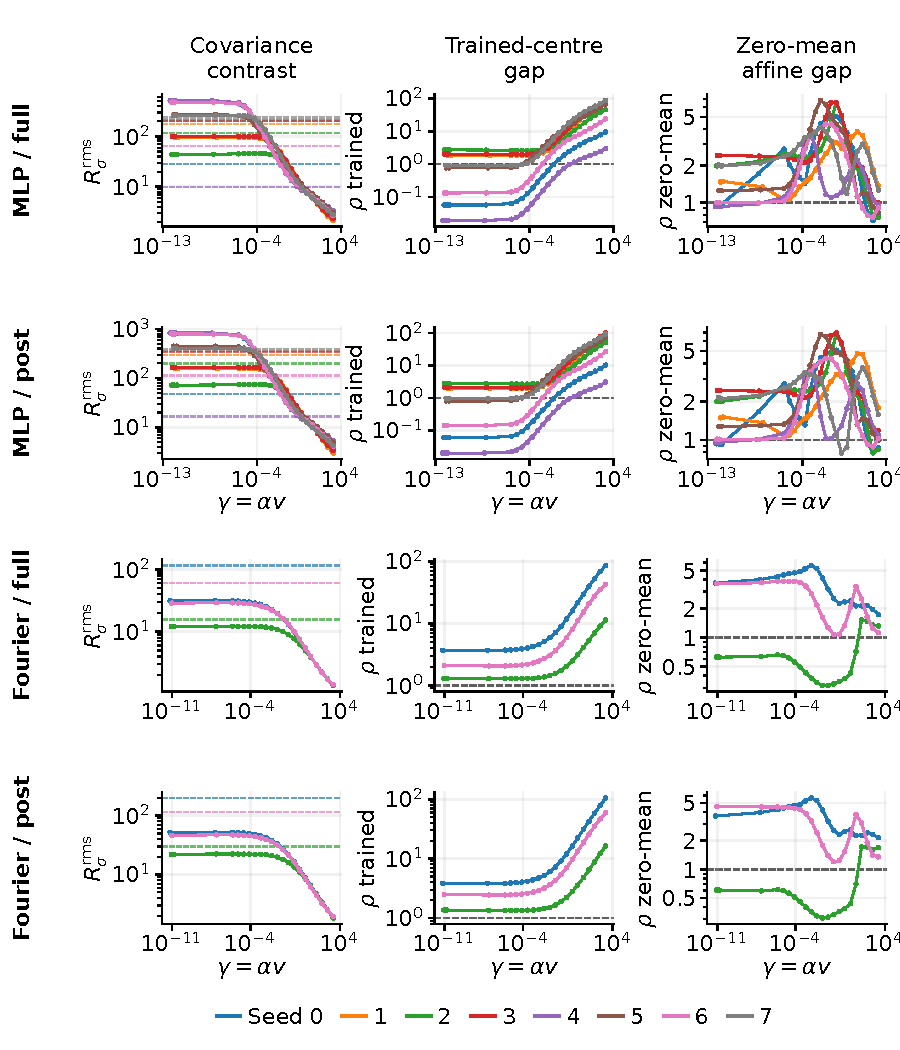
\includegraphics[width=.95\textwidth]{figures/round2_burgers_families_merged.pdf}
\caption{Burgers: eight admitted MLP and three admitted Fourier runs. Rows show MLP
full-grid/post-formation, then Fourier full-grid/post-formation; post-formation
intersects unchanged global masks with $t\ge1/\pi$. Columns show RMS covariance
contrast, trained gap and zero-mean affine gap; each gap uses its centre's error target.
Coloured dashed lines give trained error targets; grey lines mark $\rho=1$.
Every distinct saved $\gamma$, including extensions and sensitivity aliases, uses the
original Jacobian. Lines join samples without establishing monotonicity or a weak limit.}
\label{fig:r2-full-burgers}\label{fig:r2-full-bf}
\label{fig:r2-post-bm}\label{fig:r2-post}
\end{figure}

\clearpage
\begin{figure}[!tbp]
\centering
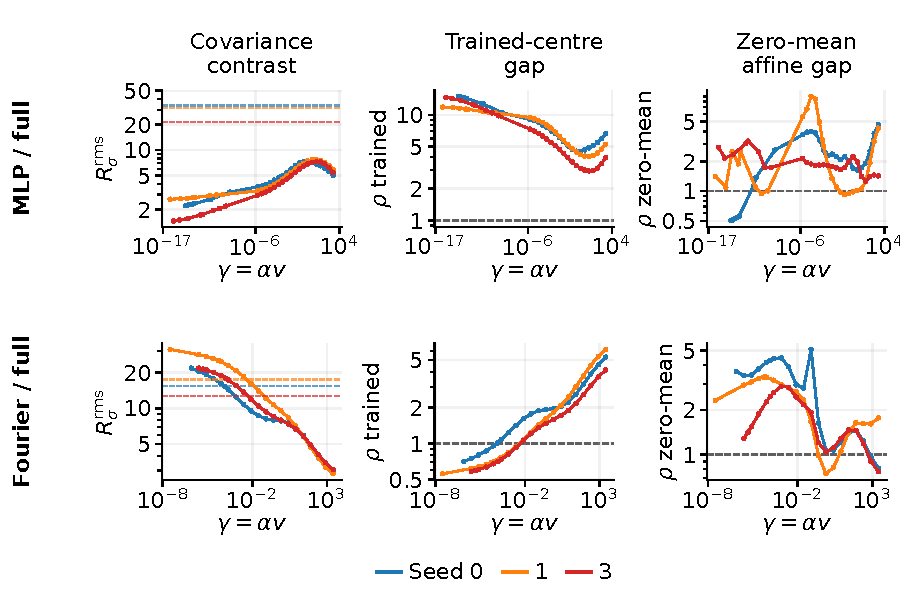
\includegraphics[width=.98\textwidth]{figures/round2_allen_cahn_families_merged.pdf}
\caption{Allen--Cahn full-grid scale and centre curves for three admitted MLP (top)
and three admitted Fourier (bottom) checkpoints. Columns and dashed lines follow
Figure~\ref{fig:r2-full-burgers}; each gap uses its centre's error target. Evidence
settings for both families are in Table~\ref{tab:r2-evidence}. All panels use the
original Jacobian; lines connect saved settings.}
\label{fig:r2-full-ac}\label{fig:r2-full-af}
\end{figure}
